Algorithm:
\begin{itemize}
	\item Start with the all-zero flow
	\item Let current flow be $f$.
	\item Construct residual graph $G_f$.
	\item While there is a path from $s$ to $t$ in $G_f$.
	\begin{itemize}
		\item Find a flow $f_1$ on such a path (limited by min capacity on path)\item Set new flow to be $f = f + f_1$
		\item Construct new residual graph $G_f$.
	\end{itemize}
\end{itemize}

Easy to see that the algorithm only produces feasible flows.

The following is an example. It turns out that the algorithm is not so fast and it could repeatedly take a path involving the middle edge and only be able to augment the flow value by 1 per iteration.
\begin{figure}[H]
	\centering
	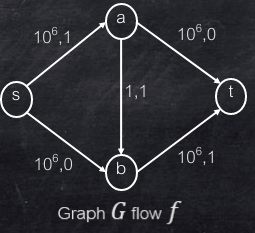
\includegraphics[width=0.3\textwidth]{fig/runtime.png}
\end{figure}
It will take 2-million iterations to arrive at the flow value of 2 million. This is not efficient because capacity $n$ can be represented by $\log n$ input bits. But if the capacities are small integers, then this algorithm is okay.

